\documentclass[__main__.tex]{subfiles}

\begin{document}
\paragraph{О-05}
Точечный источник монохроматического света помещен на расстоянии $a$ от круглой диафрагмы, а экран с противоположной стороны - на расстоянии $b$ от нее. При каких радиусах диафрагмы $r$ центр дифракционных колец, наблюдаемых на экране, будет темным и при каких - светлым, если перпендикуляр, опущенный из источника на плоскость диафрагмы, проходит через ее центр?\\

Освещенность в центре дифракционной картины можно найти, разбивая волновую поверхность $ACB$ на зоны Френеля. Если в ней уложится четное количество зон Френеля, то в точке $P$ получится минимум освещенности, если нечетное -- максимум. Построим сферу радиуса $PA$ с центром в точке $P$. Число зон Френеля на волновой поверхности $ACB$, очевидно равно длине $CD$, деленной на $\dfrac{\lambda}{2}$. Отсюда легко получить, что $r=\sqrt{\dfrac{m\lambda}{1/a+1/b}}$. Центр колец темный, если $m$ -- четное число, и светлый, если $m$ -- нечетное.
$$
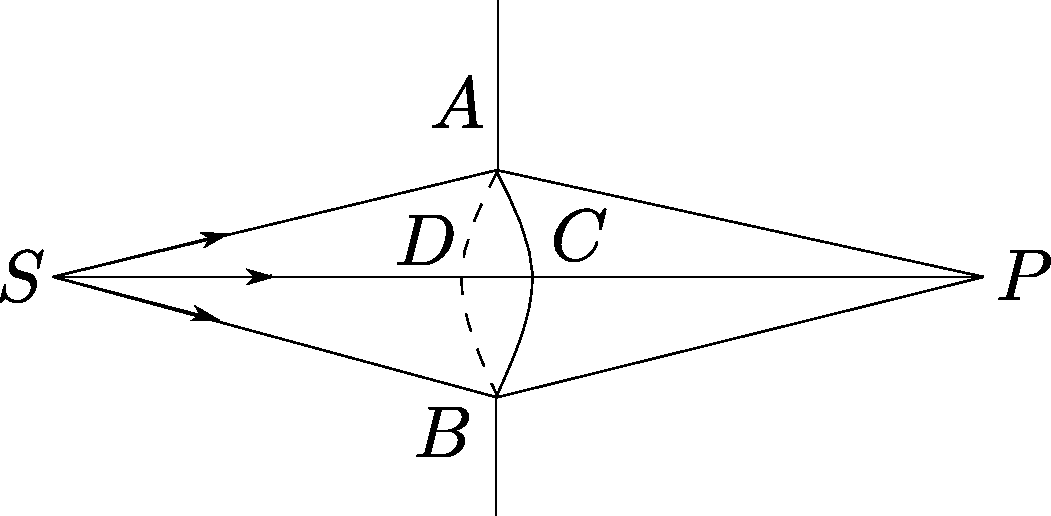
\includegraphics[scale=0.5]{img/o05.pdf}
$$

ПыСы Это решение из решебника какого-то задачника. Вроде очевидно, что верно там все говорится, но как получается эта формула --- не ебу
\end{document}